\chapter{基于树形条件随机场的高效依存句法分析}
本章首先分析了第\ref{sec:super_tc}章提出的树库转化方法和树库融合方法的不足之处,然后针对这两方面进行改进.
一方面,为了深度、高效地编码源端句法树,我们改进基于SP-TreeLSTM方法,并提出基于Full-TreeLSTM的树库转化方法,提升了转化模型的速度和性能;
另一方面,为了缓解转化后树库中存在的噪音问题,我们尝试了两种简单有效的树库融合方法,即语料加权方法以及合并后微调方法,更加合理地使用了转化后树库,进一步提升了目标端句法模型的性能.
%最后,相较于之前树库转化方法的级联模型,我们提出一种更为简洁的耦合性更强的基于多任务学习的依存句法-树库转化的联合模型.
%除了利用上一章的转化数据$CODT^{\texttt{PCTB7}}$
最后,为了得到更可靠的实验结果和结论,我们额外构建了一份双树对齐数据$CODT^{\texttt{PCTB7}}$,本章所有的方法均在两份转化语料上进行实验.

\section{引言}
\input{figures/dep-example.tex}
依存句法分析任务是NLP领域的一个基础性任务,由于其简洁性,以及可以方便的在多语言上获得句法和语义信息的特性,目前在这一任务上已经有了大量的研究. 如图\ref{fig:dep-tree-example}所示,给定一个句子$\boldsymbol{x}=w_0w_1\cdots w_n$,一棵依存树被定义为$\boldsymbol{y}=\{(i,j,l),0\le i \le n,1 \le j \le n,l \in \mathcal{L}\}$,其中$(i,j,l)$是一条从头(head)$w_i$到修饰词(modifier)$w_j$的弧,弧的标签为$l \in \mathcal{L}$. 目前在依存句法分析任务上有两个主流方法,分别是基于转移(transition-based)的方法,和基于图(graph-based)的方法,这里我们的方法主要关注于基于图的解析方式.

在深度学习时代之前,基于图的解析依赖于很多手工特征的设计,比如词性、前缀、后缀等等.
与神经网络方法相比,以前的方法有两个显著的不同.
首先,对于非神经网络方法而言,结构化学习(结构化学习)是不可或缺的,即训练时需要显式地建模树结构的约束.
通常此类方法采用的是max-margin训练算法,首先用当前模型训练一棵分值最高的树,然后更新模型参数,以保证正确的树的分值要高于预测树.

第二个显著的区别在于高阶特征的使用. 高阶特征为模型带来了显著的提升.
基础的一阶模型将句法树的分值分解为若干条独立的弧的分值\cite{mcdonald-etal-2005-online}. 后续的工作进一步引入了二阶依存弧对对分值,比如邻接兄弟\cite{mcdonald-pereira-2006-online}和祖父-父亲-孩子这样的弧对\cite{carreras-2007-experiments,koo-collins-2010-efficient},这些高阶扩展都带来了模型性能的显著提升\footnote{三阶和四阶模型的提升不大,这可能是由于特征稀疏的问题导致的\cite{koo-collins-2010-efficient,ma-zhao-2012-fourth}.}. 但是这些高阶模型需要引入更复杂的解码算法,导致了模型更加低效.


相比之下,基于图的神经网络依存句法分析器的发展呈现出相反的趋势.
\cite{pei-etal-2015-effective}提出利用前馈神经网络来自动学习\cite{chen-manning-2014-fast}的若干特征组合,并计算子树得分.
他们的工作表明引入二阶邻接兄弟子树的分值显著提高了性能。
随后,\cite{wang-chang-2016-graph}和\cite{kiperwasser-goldberg-2016-simple}都建议使用BiLSTM作为编码器和,以及在一阶模型中利用minus-feature来对单条弧打分.
这三个代表性方法都采用了全局的max-margin方法.
\cite{Timothy-d17-biaffine}提出了一种强大而高效的Biaffine Parser,并在各种数据集和语言上获得了最先进的精度.
Biaffine Parser也是一阶的,通过对每个词进行局部头选择(head selection)的方式\cite{zhang-etal-2017-dependency-parsing},采用了更简单、更有效的非结构化训练方法.

基于这些对比,我们尝试在基于图的解析器的基础上,将前深度学习时代的一些方法与神经网络模型做一下连接.
这里要解决的\textbf{第一个问题}是:
\emph{以前的一些技术,比如结构化学习和高阶建模,能够进一步提升当前最佳的解析器Biaffine Parser的性能吗\footnote{
        尽管最近的一些工作汇报了相比Biaffin Parser更高的性能,但是都引入了一些外部资源,比如大规模语言模型的上下文词表示. 在相同网络和相同实验设置的场景下,这些工作的结果都是相近的.
    },如果可以,他们在哪些方面是有用的?}

对于结构化学习而言,相比max-margin方法,我们采用更复杂且更不常用的TreeCRF.
主要原因有两方面.
首先,概率分布估计一直是当前数据驱动的NLP方法的一个核心的问题\cite{le-zuidema-2014-inside}.
如果将解析器的输出应用到更高层的任务,一棵句法树的概率$p(\boldsymbol{y}\mid\boldsymbol{x})$比没有上下边界的分值$s (\boldsymbol{x},\boldsymbol{y})$一般而言要更加有用.
其次,边缘概率是一种理论上比较可靠的方法来评估模型输出子树的置信度,可以用于最小贝叶斯风险(MBR)解码\cite{smith-smith-2007-probabilistic},并且已经被证明了对于词级别基于局部标注句法树的主动学习(active learning)\cite{li-etal-2016-active}很有用.

尽管很有用,但是TreeCRF不如max-margin那么留下,其中一个原因是由于inside-outside算法的高复杂度,尤其是outside算法.
据我们所知,所有现存的模型都是在CPU上运算inside-outside算法.
而由于CPU/GPU巨大的效率差异,这一低效的问题在深度学习时代变得更加严重.
这就引发了\textbf{第二个问题}:
\emph{我们是否能够批次化inside-outside算法,并且直接在GPU上进行计算?}
如果这样的话,我们就能够利用诸如PyTorch这样的高效深度学习张量库来进行计算,并且将高效的TreeCRF应用到更多的场景\cite{cai-etal-2017-crf,le-zuidema-2014-inside}.

总体而言,针对上面的两个问题,我们做了下面的几个贡献:
\begin{itemize}%[leftmargin=10pt,topsep=3pt,itemsep=1pt,partopsep=1pt]
    \item 我们第一次提出了将二阶TreeCRF应用到神经依存句法分析中.
          我们还提出了一个高效的Triaffine结构来对于二阶子树打分.
    \item 我们提出通过GPU上大规模的并行张量计算来批次化inside算法,来进行更高效的TreeCRF损失函数的计算.
          我们表明复杂的outside算法对于梯度和边缘概率的计算而言已不再必须,相应的可以用高效的反向传播代替.
    \item 我们在13个语言的27个树库上进行了实验.
          结果和分析都表明,深度学习时代的,结构化学习和高阶建模在许多方面对当前最好的Biaffine Parser仍然是有用的.
\end{itemize}

\section{基线模型}
\label{section:basic_model}


We re-implement the state-of-the-art biaffine parser \cite{Timothy-d17-biaffine} with
% We follow their work in all important details such as dropouts and initialization.
two modifications, i.e., using CharLSTM word representation vectors instead of POS tag embeddings, and
the first-order Eisner algorithm \cite{eisner-2000-iwptbook}
for projective decoding instead of the non-projective MST algorithm.

\paragraph{Scoring architecture.}
%(Figure~\ref{fig:biaffine-parser-architecture})}
Figure~\ref{fig:framework} shows the scoring architecture, consisting of four components.

% The basic architecture of our model is mainly based on that of .
% In this section, we describe the components of the basic parsing model in a top-down fashion.

% We then introduce the scoring functions which are capable of capturing the relations of head-modifier pairs or even higher order.

%We first have a review of the word encoding part.

% 先别删这句话:最后的数学符号要过一遍,统一一下,严谨!粗体、斜体、大小写等

\subparagraph{Input vectors.}
The $i$th input vector % for the $i$th word
is composed of two parts:
the word embedding and the CharLSTM word representation vector of $w_i$.
\begin{equation}
    \label{equation:input}
    \mathbf{e}_i=\mathrm{emb}({w_i}) \oplus \mathrm{CharLSTM}(w_i)
\end{equation}
where $\mathrm{CharLSTM}(w_i)$ is obtained by feeding $w_i$ into a BiLSTM and
then concatenating the two last hidden vectors \cite{lample-etal-2016-neural}.
We find that replacing POS tag embeddings with  $\mathrm{CharLSTM}(w_i)$ leads to consistent improvement,
and also simplifies the multilingual experiments by avoiding POS tag generation (especially n-fold jackknifing on training data).
%Compared with POS tag embeddings, we find that
%where $\mathbf{e}_i$ is the concatenation of the word embedding $\mathbf{e}_i^{w}$ and character-level embedding $\mathbf{e}_i^{c}$.
%$\mathbf{e}_i^{c}$ is acquired by concatenating the last hidden states produced by the BiLSTM performing on the word characters \cite{lample-etal-2016-neural}.

%Since subsequent researchers have show the effectiveness of character-level embeddings \cite{dozat-etal-2017-stanfords,kitaev-klein-2018-constituency},
%we make a few modifications for the input that replacing the Part-of-Speech (POS) Tag embeddings with \textsc{CharLSTM} word representations.
%Given a sentence $\boldsymbol{x}=w_0,w_1, \ldots, w_n$, where $w_0$ denotes the root node, each word $w_i$ is mapped into a dense vector $\mathbf{e}_i$
% \footnote{
% We adopt the convention of \citet{Timothy-d17-biaffine} that uses lowercase italics for scalars, lowercase bold for vectors, uppercase italics for matrices, and uppercase bold for tensors.
% },

\subparagraph{BiLSTM encoder.} To encode the sentential contexts,
the parser applies three BiLSTM layers %are applied
over %the input vector sequence
$\mathbf{e}_0 \dots \mathbf{e}_n$. The output vector of the top-layer BiLSTM for the $i$th word
is denoted as $\mathbf{h}_i$.
%The $i$th
%Then we use the corresponding hidden output for parsing, denoted as $\mathbf{r}_i$.
%We use  to denote .

\subparagraph{MLP feature extraction.} Two shared MLPs are applied to $\mathbf{h}_i$, obtaining
two lower-dimensional vectors that detain only syntax-related features:
\begin{equation}
    \label{mlp-arc}
    %\mathbf{r}_i^{h}; \mathbf{r}_i^{m} =\mathrm{MLP}_{h/m} (\mathbf{h}_i);\mathrm{MLP}_{m} (\mathbf{h}_i)
    \mathbf{r}_i^{h}; \mathbf{r}_i^{m} =\mathrm{MLP}^{h/m} \left( \mathbf{h}_i \right)
\end{equation}
where $\mathbf{r}_i^{h}$ and $\mathbf{r}_i^{m}$ are the representation vector of $w_i$ as a head word and a modifier word respectively.


\subparagraph{Biaffine scorer.}
%Biaffine计算效率很高。
%Recent works regard graph-based dependency parsing as a head selection task \cite{zhang-etal-2017-dependency-parsing,Timothy-d17-biaffine}.
%For each word pair ($w_i$, $w_j$), they assign it a score to measure how possible the word $w_j$ modifies $w_i$,
%and select the one with the highest score one as the resulting head-dependent pair.
%As a representative job,
\citet{Timothy-d17-biaffine} for the first time propose to compute the score of a dependency $i \rightarrow j$ via biaffine attention:
%  design a very subtle biaffine operation.
\begin{equation} \label{equation:biaffine}
    %score(i, j) =  \big[{{\mathbf r_i^{D}} \oplus {\mathbf{1}}} \big]^\textup T   W^b  \mathbf r_j^{H}
    s(i,j) =  \left[
        \begin{array}{c}
            \mathbf{r}_{j}^{m} \\
            1
        \end{array}
        \right]^\mathrm{T}
    \mathbf{W}^\textit{biaffine}  \mathbf{r}_{i}^{h}
\end{equation}
where $\mathbf{W}^\textit{biaffine} \in \mathbb{R}^{d \times d}$.
The computation is %straightforward to batchify on GPUs and thus
extremely efficient on GPUs.
%Specifically, they first apply MLP layers on $\mathbf{r}_i$ to obtain the representations of each word as a head ($\mathbf{h}_i^{arc}$) and as a dependent ($\mathbf{d}_i^{arc}$):
%As discussed in \citet{Timothy-d17-biaffine}, the MLP layers on the one hand reduces the dimensionality of $\mathbf{r}_i$,
%and more importantly on the other hand strips away syntax-unrelated information and thus avoids the risk of over-fitting.


\begin{figure}[tb]
    \centering
    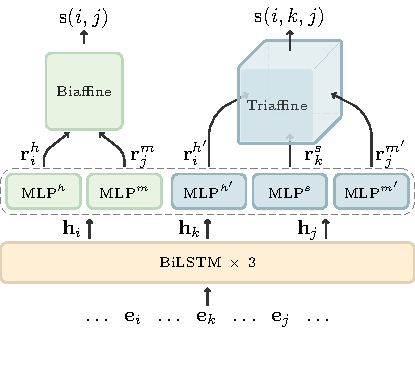
\includegraphics{figures/framework.pdf}
    \caption{Scoring architecture with second-order extension.
        %可否把7个MLP都画出来,然后label部分的biaffine画成层叠的,表示有多个。
        %不,就画5个,我会在正文中专门讲label的处理;
        %然后biaffine和triaffine输出加上$\mathrm{s}(i,j,l)$, $\mathrm{s}(i,j)$, $\mathrm{s}(i,k,j)$等
    }
    \label{fig:framework}
    % \vspace{-5pt}
\end{figure}

\paragraph{Local token-wise training loss.}
The biaffine parser adopts a simple non-structural training loss,
trying to independently maximize the local probability of the correct head word for each word.
%For a gold-standard dependency $i \rightarrow j$
For a gold-standard head-modifier pair ($w_i$, $w_j$)
in a training instance,
%For $w_j$ and its gold-standard head $w_i$,
the cross-entropy loss is
\begin{equation} \label{equation:biaffine-loss}
    \mathit{L}(i,j) = -\log{\frac{e^{s(i,j)}}{\sum_{0 \le k \le n} e^{s(k,j)}}}
    % & -\log{
    % \frac{e^{\texttt{score}(i \xleftarrow{l} j)}}
    % {\sum_{l' \in \mathcal{L}} e^{\texttt{score}(i \xleftarrow{l'} j)}}
    % }
\end{equation}
%where $\mathcal{L}$ is the label set.
In other words, the model is trained based on simple head selection,
without considering the tree structure at all, and
losses of all words in a mini-batch are accumulated.

\paragraph{Decoding.} Having scores of all dependencies,
we adopt the first-order Eisner algorithm with time complexity of $O(n^3)$
to find the optimal tree.
\begin{equation}
    \label{equation:map-decoding}
    {\boldsymbol{y}}^* = \arg\max_{\boldsymbol{y}} \left[ s(\boldsymbol{x},\boldsymbol{y}) \equiv
        %& s(\boldsymbol{x},\boldsymbol{y}) =
        \sum_{i \rightarrow j \in \boldsymbol{y}}{s(i,j)} \right]
\end{equation}
% 这段话考虑移到其他地方。
% Since this work focuses on projective dependency parsing,
% we adopt the pseudo-projective approach \cite{nivre-nilsson-2005-pseudo} for handling non-projective datasets. % with non-projective trees.
% The idea is to transform non-projective trees in projective ones using more complex labels for post-processing recovery.

\paragraph{Handling dependency labels.}
The biaffine parser treats skeletal tree searching and labeling as two independent (training phase) and cascaded (parsing phase) tasks.
This work follows the same strategy for simplicity. Please refer to \citet{Timothy-d17-biaffine} for details.

% Then a biaffine layer is used to compute scores of all dependencies.
% For pair ($i$, $j$), the score function $\mathrm{s}(i, j)$ is defined as
% \begin{equation}
% \mathrm{s}(i, j)=\mathbf{h}_i^{T}W\mathbf{d}_j+\mathbf{u}^T\mathbf{h}_i
% \end{equation}
% where $W \in \mathbb{R}^{d \times d}$ and $\mathbf{u}$ are weight parameters. For simplicity, we omit some superscripts in the formula.

% For dependency labels, extra MLP and Biaffine layers are used to compute the scores $\mathrm{s}(i, j, l)$, where $l$ is the label on the edge ($w_i$, $w_j$)
% We omit the details for brevity.

% During training, for the gold head-dependent pair ($w_i$, $w_j$) , we use the cross-entropy loss to maximize the probability of $w_i$ being the head against all
% words, i.e.,
% $\frac{\exp \mathrm{s}(i, j)}{\sum_{0 \le j^{\prime} \le n} \exp \mathrm{s}(i, j^{\prime})}$.

% \paragraph{Decoding.}
% To ensure well-formedness, we follow two strategies of prior works.
% For treebanks like PTB that contains very few non-projective arcs, we apply the Eisner algorithm to form a valid tree.
% For treebanks that contain a lot of non-projective arcs, we first convert them to pseudo-projective and then apply the Eisner algorithm.
% We have also tried the mst algorithm used in \citet{Timothy-d17-biaffine}. Results show that it is slightly inferior to pseudo-projective ones.
% We leave detailed discussions in Section \ref{section:experiments-analysis}.


% \begin{figure}[tb]
% \subfigure[single dependency] {
%   \begin{minipage}[b]{0.22\textwidth}
%   \centering
%   \includegraphics{figures/scoring-part/a.pdf}
%   \label{fig:scoring-part-a}
%   \end{minipage}
% }
% \subfigure[adjacent sibling] {
%   \begin{minipage}[b]{0.22\textwidth}
%   \centering
%   \includegraphics{figures/scoring-part/b.pdf}
%   \label{fig:scoring-part-b}
%   \end{minipage}
% }
% \caption{The two types of scoring subtrees.}
% \label{fig:scoring-part}

\section{Second-order TreeCRF}
\label{2o-tree-crf}

%\citet{Timothy-d17-biaffine} only take into account the first-order part, i.e., the head-dependent relation in their parsing system.
%Recently, several fruitful investigations have been made on integrating higher-order structured features \cite{mcdonald-pereira-2006-online,carreras-2007-experiments,koo-collins-2010-efficient,ma-zhao-2012-fourth}.
%Considering that their architectures might not be competitive with the current state-of-the-art work, in this paper, we extend the biaffine parser by utilizing high-order parts.

This work substantially extends the biaffine parser in two closely related aspects:
using probabilistic TreeCRF for structural training and explicitly incorporating high-order subtree scores.
%using probabilistic TreeCRF for structural training, and incorporating second-order modeling.
%First, under the second-order modeling,
Specifically, we further incorporate adjacent-sibling subtree scores into the basic first-order model:\footnote{
    This work can be further extended to incorporate
    grand-parent-modifier subtree scores
    %can be realized based on the techniques presented in this work
    %by extending
    based on the viterbi algorithm of $O(n^4)$ time complexity proposed by \citet{koo-collins-2010-efficient}, which
    %, requiring
    we leave for future work.
}
%the score of a tree
\begin{equation}\label{eq:score-definition-2o}
    s(\boldsymbol{x}, \boldsymbol{y}) = \sum_{i\rightarrow j \in \boldsymbol{y}}s(i,j) + \sum_{
        %\begin{array}{c}
        i\rightarrow \{k,j\} \in \boldsymbol{y} %\
        %  i\rightarrow k \in \boldsymbol{y}
        %\end{array}
    } s(i,k,j)
\end{equation}
where $k$ and $j$ are two adjacent modifiers of $i$ and satisfy either $i < k < j$ or $j < k < i$.
%s(\boldsymbol{x}, \boldsymbol{y}) = \sum_{i\rightarrow j \in \boldsymbol{y}}

As a probabilistic model, TreeCRF computes the conditional probability of a tree as
\begin{equation}\label{equation:prob-labeled}
    \begin{split}
        & p(\boldsymbol{y}\mid\boldsymbol{x})  = \frac{e^{s(\boldsymbol{x},\boldsymbol{y})}}{Z(\boldsymbol{x}) \equiv \sum_{\boldsymbol{y'} \in \mathcal{Y}(\boldsymbol{x})} {e^{s(\boldsymbol{x},\boldsymbol{y'})}}}
    \end{split}
\end{equation}
where $\mathcal{Y}(\boldsymbol{x})$ is the set of all legal (projective) trees for $\boldsymbol{x}$, and
$Z(\boldsymbol{x})$ is commonly referred to as the normalization (or partition) term.

During training, TreeCRF employs the following structural training loss to
maximize the conditional probability of the gold-standard tree $\boldsymbol{y}$ given $\boldsymbol{x}$.
\begin{equation}\label{equation:training-loss-treecrf}
    \begin{split}
        \mathit{L}(\boldsymbol{x},\boldsymbol{y}) &= -\log p(\boldsymbol{y}\mid\boldsymbol{x})  \\
        &= - s(\boldsymbol{x}, \boldsymbol{y}) + \log Z(\boldsymbol{x})
    \end{split}
\end{equation}

\begin{figure}[tb]
    \centering
    \begin{subfigure}[b]{\textwidth}
        \begin{minipage}{\textwidth}
            \centering
            \includegraphics{figures/eisner-2o/a.pdf}
            \label{fig:eisner-2o-a}
        \end{minipage}
    \end{subfigure}
    \begin{subfigure}[b]{\textwidth}
        \begin{minipage}{\textwidth}
            \centering
            \includegraphics{figures/eisner-2o/b.pdf}
            \label{fig:eisner-2o-b}
        \end{minipage}
    \end{subfigure}
    \begin{subfigure}[b]{\textwidth}
        \begin{minipage}{\textwidth}
            \centering
            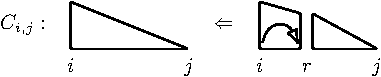
\includegraphics{figures/eisner-2o/c.pdf}
            \label{fig:eisner-2o-c}
        \end{minipage}
    \end{subfigure}
    \caption{基于自底向上动态规划的二阶Inside算法图示.}
    \label{fig:eisner-2o}
    % \vspace{-5pt}
\end{figure}

\subsection{Scoring Second-order Subtrees}
To avoid major modification to the original scoring architecture,
we take a straightforward extension to obtain scores of adjacent-sibling subtrees.
First, we employ three extra MLPs to perform similar feature extraction.
\begin{equation}
    \label{mlp-sib}
    \mathbf{r}_i^{h'}; \mathbf{r}_i^{s}; \mathbf{r}_i^{m'} =\mathrm{MLP}^{h'/s/m'} \left( \mathbf{h}_i \right)
\end{equation}
where $\mathbf{r}_i^{h'}; \mathbf{r}_i^{s}; \mathbf{r}_i^{m'}$ are the representation vectors of $w_i$ as
head, sibling, and modifier respectively.\footnote{
    %We find re-using head and modifier representations from the basic first-order component leads to inferior performance,
    %indicating it is better to
    Another way is to use one extra MLP for sibling representation, and re-use head and modifier representation from the basic first-order components, which however leads to inferior performance
    in our preliminary experiments.
    % indicating that it is better
    % possibly due to the confusion.
    %, possibly due to  ??
    % 效率问题,那个太大了。
}

% Note that in \citet{wang-etal-2019-second}'s paper, they use the product of three rank-2 matrices to simulate the rank-3 $\mathbf{W}$ in order to reduce the  computation cost.
% We discard this trade-off because Equation~\ref{equation:triaffine} is more accurate and our implementation is efficient enough to do the computation
% \footnote{We implement the triaffine by the very efficient $\mathrm{einsum}$ operation.}.
% Detailed discussions are available at Section \ref{section:experiments-analysis}.


Then, we
propose a natural extension to the biaffine equation, and employ triaffine for score computation over three vectors.\footnote{
    We have also tried the approximate method of \citet{wang-etal-2019-second}, which uses three
    biaffine operations to simulate the interactions of three input vectors, but observed inferior performance.
    We omit the results due to the space limitation.
}
%, analogous to the biaffine equation.
\begin{equation} \label{equation:triaffine}
    %score(i, j) =  \big[{{\mathbf r_i^{D}} \oplus {\mathbf{1}}} \big]^\textup T   W^b  \mathbf r_j^{H}
    s(i,k,j) =
    \left[
        \begin{array}{c}
            \mathbf{r}_{k}^{s} \\
            1
        \end{array}
        \right]^\mathrm{T}
    {\mathbf{r}_{i}^{h'}}^\mathrm{T}
    \mathbf{W}^\textit{triaffine}
    \left[
        \begin{array}{c}
            \mathbf{r}_{j}^{m'} \\
            1
        \end{array}
        \right]
\end{equation}
where $\mathbf{W}^\textit{triaffine} \in \mathbb{R}^{d' \times d' \times d'}$ is a three-way tensor.
%We find that
The triaffine computation can be quite efficiently performed with the $\mathrm{einsum}$ function on PyTorch.
% 下面这些话不知道是否要讲。
%Due to GPU memory limitation for most our machines, we set $d'=100$ (versus $d=500$ in $\mathbf{W}^\textit{biaffine}$) and
%However, experiments with $d'=300$ on computers with larger GPUs shows little performance boost.

%Specifically, we incorporate relations of siblings.
% We use the second-order score function $\mathrm{s}(i, k, j)$ to draw the relation of a word triple ($w_i$, $w_k$, $w_j$),
% where $w_k$ and $w_j$ are adjacent, same-side dependents and modify the common head $w_i$ \cite{mcdonald-pereira-2006-online}. Figure~\ref{fig:scoring-part} shows the relations.
% To better distinguish their roles, similar to Equation~\ref{mlp-arc}, we apply extra MLP layers to extract the representations:


% \begin{equation}
% \mathbf{h}_i^{sib}; \mathbf{d}_i^{sib}; \mathbf{s}_i^{sib} =\mathrm{MLP}^{sib} \left(\mathbf{r}_i \right)
% \end{equation}
% $\mathbf{h}_i^{sib}$, $\mathbf{d}_i^{sib}$ and $\mathbf{s}_i^{sib}$ are  representations of the head, dependent and the second-order part, respectively.
% Then, inspired by \citet{wang-etal-2019-second}, we adopt the following triaffine score function:
% \begin{equation}
% \label{equation:triaffine}
% \mathrm{s}(i, k, j)=\mathbf{h}_i^{T}\mathbf{s}_k^{T}\mathbf{W}\mathbf{d}_j+\mathbf{h}_i^{T}U+ \mathbf{d}_j^{T}V+\mathbf{b}
% \end{equation}

% we regard each sibling as a special label and model the likelihood of such label given both the word $w_j$ and its head $w_i$.
% Detailed interpretation of the meaning of $\mathbf{W} \in \mathbb{R}^{d \times d \times d}$, $U$, $V$ and the bias term $\mathbf{b}$ is analogous to that of \citet{Timothy-d17-biaffine}.


%\subsection{TreeCRF Training Loss}

\subsection{Computing TreeCRF Loss Efficiently}

% One major shortcoming of \citet{Timothy-d17-biaffine} is that their training objective is confined to the head-selection.
% Though simple and effective enough, some global structured information might be lost during the training process.

The key to TreeCRF loss is how to efficiently compute $\log Z(\boldsymbol{x})$,
as shown in Equation~\ref{equation:training-loss-treecrf}.
This problem has been well solved long before the DL era
for non-neural dependency parsing.
Straightforwardly, we can directly extend the viterbi decoding algorithm by replacing max product with sum product, and naturally obtain $\log Z(\boldsymbol{x})$ in the same polynomial time complexity.
%However, previous works non-neural parsing
However, it is not enough to solely perform the inside algorithm for non-neural parsing, due to the inapplicability of the automatic differentiation mechanism. %which is an obvious advantage in the DL era as shown in this work
In order to obtain marginal probabilities and then feature weight gradients, we have to realize the more sophisticated outside algorithm, which is usually at least twice slower than the inside algorithm.
%All these factors lead to
This may be the major reason for the less popularity of TreeCRF (vs. max-margin training) before the DL era.

\begin{algorithm}[tb]
    \begin{algorithmic}[1]
        \newlength{\commentindent}
        \setlength{\commentindent}{.3\textwidth}
        \renewcommand{\algorithmiccomment}[1]{\unskip\hfill\makebox[\commentindent][l]{$\rhd$~#1}\par}
        \LetLtxMacro{\oldalgorithmic}{\algorithmic}
        \renewcommand{\algorithmic}[1][0]{
            \oldalgorithmic[#1]
            \renewcommand{\ALC@com}[1]{
                \ifnum\pdfstrcmp{##1}{default}=0\else\algorithmiccomment{##1}\fi}%
        }
        \STATE \textbf{define:} $I,S,C \in \mathbb{R}^{n \times n \times B}$ \COMMENT{$B$ is \#sents in a batch}
        \STATE \textbf{initialize:} $C_{i, i}  = 0, 0 \le i \le n$

        \FOR [span width]{$w = 1$ \TO $n$}
        \STATE \textbf{Batchify:} $0 \le i$; $j=i+w \le n$
        \STATE $I_{i, j} = \log\left(\exp\left(C_{i, i}  +  C_{j, i+1}\right) ~ +\sum\limits_{i < r < j} \exp\left(I_{i, r} + S_{r, j}+ \mathrm{s}(i, r, j)\right)\right) + \mathrm{s}(i, j)$
        \STATE $S_{i, j} = \log \sum\limits_{i \le r < j} \exp\left(C_{i, r}  +  C_{j, r+1}\right) $ \\
        \STATE $C_{i, j} = \log \sum\limits_{i < r \le j} \exp\left(I_{i, r}  +  C_{r, j}\right)  $ \\
        \ENDFOR \COMMENT{refer to Fig.~\ref{fig:eisner-2o}}
        \RETURN $C_{0, n} \equiv \log Z(\boldsymbol{x})$
    \end{algorithmic}
    \caption{二阶Inside算法.}
    \label{alg:eisner-2o}
\end{algorithm}


As far as we know, all previous works on neural TreeCRF parsing
explicitly implement the inside-outside algorithm for gradient computation \cite{zhang-etal-2019-empirical, jiang-etal-2018-supervised}.
To improve efficiency, computation is transferred from GPUs to CPUs with Cython programming.

This work shows that the inside algorithm
can be effectively batchified to fully utilize the power of GPUs.
Figure~\ref{fig:eisner-2o} and Algorithm \ref{alg:eisner-2o} together illustrate the batchified version of the second-order inside algorithm, which is a direct extension of the second-order Eisner algorithm in \citet{mcdonald-pereira-2006-online} by replacing max product with sum product.
We omit the generations of incomplete, complete, and sibling spans in the opposite direction from $j$ to $i$ for brevity.

% shows the bottom-up operations
% used in both the inside algorithms, and Algorithm
% \ref{alg:eisner-2o}
% present the batchified inside algorithm.

% Specifically, we extend the second-order Eisner algorithm described in \citet{mcdonald-pereira-2006-online} into the inside algorithm.
% Figure~\ref{fig:eisner-2o} shows the bottom-up operations
% used in both the inside and decoding algorithms, and Algorithm
% \ref{alg:eisner-2o}
% present the batchified inside algorithm. To save space, we omit the generations of reverse structures from $j$ to $i$.

Basically, we first pack the scores of same-width spans at different positions
($i, j$) for all $B$ sentences in the data batch into large tensors.
Then we can do computation and aggregation simultaneously on GPUs via efficient large tensor operation.
% Meanwhile, elaborately masking is needed to skip illegal operations not allowed in Figure~\ref{fig:eisner-2o}.

Similarly, we also batchify the decoding algorithm. Due to space limitation, we omit the details.

It is noteworthy that the techniques described here are also applicable to other grammar formulations such as CKY-style constituency parsing \cite{finkel-etal-2008-efficient,drozdov-etal-2019-unsupervised-latent}.

%  since
% GPUs are very suitable for large tensor operation.
%  on GPUsThis leads to very efficient parallel computation on GPU
% when iterating over the width of spans, we .


% \citet{mcdonald-etal-2005-online,mcdonald-etal-2005-non} have conducted several researches in this regard.
% In this paper, we extend the biaffine biaffine by high-order structural learning based on the prior works.
% We first formula the dependency parsing as the search for the highest scoring tree from a directed graph.
% Given the sentence $\boldsymbol{x}$, the entire tree searching space $T(\boldsymbol{x})$, the score of a tree $\boldsymbol{y} \in T(\boldsymbol{x})$ is factorized into the combination of several independent subtrees.
% For first-order parsing, the subtrees are individual head-dependent pairs:
% \begin{equation}
% \label{equation:score-1o}
% \mathrm{s}(\boldsymbol{x}, \boldsymbol{y})=\sum_{(i, j) \in \boldsymbol{y}} \mathrm{s}(i, j)
% \end{equation}
% during training, we use the score to compute the probability of the tree, and take its log-linear form as the training objective
% \begin{equation}
% \label{equation:tree-prob}
% P(\boldsymbol{y}|\boldsymbol{x};\Theta)=\frac{\exp(\mathrm{s}(\boldsymbol{x}, \boldsymbol{y}))}{Z(\boldsymbol{x};\Theta)}
% \end{equation}
% where $\Theta$ is the parameters to be optimized, and
% \begin{equation}
% \label{equation:partition-fn}
% Z(\boldsymbol{x};\Theta)=\sum_{\boldsymbol{\hat{y}} \in T(\boldsymbol{x})} \exp(\mathrm{s}(\boldsymbol{x}, \boldsymbol{\hat{y}}))
% \end{equation}
% is the partition function, i.e., the summation over all possible trees in the set $T(\boldsymbol{x})$

% To maximize the probability $P(\boldsymbol{y}|\boldsymbol{x})$, we need to compute the partition function $Z(\boldsymbol{x})$.
% Though there exists exponential number of all possible trees in the searching space, the partition function can stilled be computed by the inside algorithm with the complexity of $O(n^3)$ \cite{mcdonald-pereira-2006-online},
% as illustrated in Algorithm \ref{alg:eisner-2o}. The inside is very similar to the viterbi algorithm, which only replace the $\max$ product with $\mathrm{sum}$.

% % Following prior works, researchers on the one hand continue to investigate the effectiveness of higher order global structured information \cite{mcdonald-pereira-2006-online, koo-collins-2010-efficient}.
% % On the other hand, they propose to introduce the probabilistic information to the neural network-based models \cite{ma-hovy-2017-neural,zhang-etal-2016-probabilistic}.
% % But empirical study shows that it leads to very modest improvement on the current mainstream graph-based parser \cite{zhang-etal-2019-empirical}.

% % In this paper, following \citet{zhang-etal-2019-empirical}, we make some positive exploration on the second order probabilistic parsing model.
% % by adding a \textsc{Crf} layer on top of the biaffine parser.

% % While second-order non-projective parsing is NP-hard,
% \citet{mcdonald-pereira-2006-online} have designed a second order projective parsing algorithm by incorporating siblings into the Inside algorithm \cite{eisner-2000-iwptbook}.
% In this section, we have a brief revisit.

% In the first order scenario, to facilitate an efficient and global search based on Dynamic Programming (DP) algorithm, a subtree can only correspond to an individual head-dependent pair.
% \citet{mcdonald-pereira-2006-online} intend to weaken this independence and utilize non-local features, i.e., the siblings.
% %  based on the Eisner algorithm.
% % The illustration of the DP structures behind the algorithm is shown in Figure.
% Concretely, by adding $w_k$ to the pair ($w_i$, $w_j$), forming a word triple ($w_i$, $w_k$, $w_j$), the score of tree $\boldsymbol{y}$ now becomes
% \begin{equation}
% \label{equation:score-2o}
% \mathrm{s}(\boldsymbol{x}, \boldsymbol{y})=\sum_{(i, j) \in \boldsymbol{y}} \mathrm{s}(i, j)+\sum_{(i, k, j) \in \boldsymbol{y}} \mathrm{s}(i, k, j)
% \end{equation}
% the formula relaxes the restriction of factorizing the trees into only edges and allows the interactions between adjacent siblings parts.

% In this paper, we implement a batchified version of the inside algorithm.
% Specifically, when iterating over the width of spans, we collect a batch of all the spans with the same width into a tensor and do the operation parallel.
% This leads to very efficient parallel computation on GPU.

%\subsection{Avoiding the Outside Algorithm}
\subsection{Outside via Back-propagation}

\citet{eisner-2016-inside} proposes a theoretical proof on the equivalence between
the back-propagation mechanism and the outside algorithm in the case of constituency (phrase-structure) parsing.
This work empirically verifies this equivalence for dependency parsing.
%Besides the overall parsing accuracy, In fact,
% We do find that gradient tensors are identical after running the two versions of code.

% TODO: as an empirical verification for the theoretical proposal of \citet{eisner-2016-inside} in the case of dependency parsing.
Moreover, we also find that marginal probabilities $p(i \rightarrow j\mid\boldsymbol{x})$ directly correspond to gradients after back-propagation with $\log Z(\boldsymbol{x})$ as the loss:
\begin{equation}
    \label{equation:partial-derivative}
    \begin{split}
        \frac{\partial \log Z}{\partial \mathrm{s}(i, j)} %& = \frac{\partial \log Z}{\partial Z} \cdot \frac{\partial Z}{\partial \mathrm{s}(i, j)}\\
        %  & =\frac{1}{Z} \cdot \sum_{\boldsymbol{\hat{y}}} \frac{\partial \exp \left(\mathrm{s}(\boldsymbol{x}, \boldsymbol{\hat{y}}) \right)}{\partial \mathrm{s}(i, j)}\\
        %  & =\frac{1}{Z} \cdot \sum_{\boldsymbol{\hat{y}}} \frac{\partial \exp \left( \sum_{(i^{\prime}, j^{\prime}) \in \boldsymbol{\hat{y}}} \mathrm{s}(i^{\prime}, j^{\prime}) \right)}{\partial \mathrm{s}(i, j)}\\
        %=\sum_{\boldsymbol{y}:(i,j) \in \mathbf{{y}}} \exp \left(\mathrm{s}(\boldsymbol{x}, \boldsymbol{\hat{y})} \right) \\
        % & =\frac{1}{Z} \cdot Z^{\prime} \\
        &= \sum_{\boldsymbol{y}:(i,j) \in \boldsymbol{{y}}} p(\boldsymbol{y}\mid\boldsymbol{x}) = p(i \rightarrow j\mid\boldsymbol{x})
        %\exp \left(\mathrm{s}(\boldsymbol{x}, \boldsymbol{\hat{y})} \right) \\
    \end{split}
\end{equation}
which can be easily proved. % (see Appendix).
For TreeCRF parsers, we perform MBR decoding \cite{smith-smith-2007-probabilistic} by replacing scores with marginal probabilities in the decoding algorithm,
leading to a slight but consistent accuracy increase.


% Moreover, previous works often seek to get the marginal probabilities \cite{koo-etal-2007-structured} by the classical inside-outside procedure, which is generally perceived as tricky in the project.
% Inspired by \citet{eisner-2016-inside}, we achieve this goal empirically by combining the individual inside and the back-propagation process
% \footnote{We do the back-propagation and compute the gradients very handily by the automatic differentiation mechanism in PyTorch.}.
% Concretely, given the partition function $Z(\boldsymbol{x})$, we take the gradient, i.e., the partial derivative of its log-linear form $\log Z$ with respect to the score $\mathrm{s}(i, j)$,
% as the marginal probability
% \begin{equation}
% \label{equation:grad-marg}
% P(i, j|\boldsymbol{x})=\frac{\partial \log Z}{\partial \mathrm{s}(i, j)}
% \end{equation}
% of word pair ($w_i$,$w_j$), and
% \begin{equation}
% \label{equation:partial-derivative}
% \begin{split}
% \frac{\partial \log Z}{\partial \mathrm{s}(i, j)} & =\frac{\partial \log Z}{\partial Z} \cdot \frac{\partial Z}{\partial \mathrm{s}(i, j)}\\
% & =\frac{1}{Z} \cdot \sum_{\boldsymbol{\hat{y}}} \frac{\partial \exp \left(\mathrm{s}(\boldsymbol{x}, \boldsymbol{\hat{y}}) \right)}{\partial \mathrm{s}(i, j)}\\
% & =\frac{1}{Z} \cdot \sum_{\boldsymbol{\hat{y}}} \frac{\partial \exp \left( \sum_{(i^{\prime}, j^{\prime}) \in \boldsymbol{\hat{y}}} \mathrm{s}(i^{\prime}, j^{\prime}) \right)}{\partial \mathrm{s}(i, j)}\\
% & =\frac{1}{Z} \cdot \sum_{\boldsymbol{\hat{y}}, (i,j) \in \boldsymbol{\hat{y}}} \exp \left(\mathrm{s}(\boldsymbol{x}, \boldsymbol{\hat{y})} \right) \\
% % & =\frac{1}{Z} \cdot Z^{\prime} \\
% \end{split}
% \end{equation}
% where the last item is just the definition of the marginal probability of $P(i, j|\boldsymbol{x})$. $P(i, j|\boldsymbol{x})$ is the summation of probabilities of all the trees in $T(\boldsymbol{x})$ containing the edge ($i$, $j$).


\subsection{Handling Partial Annotation}
\label{sub@section:partial-annotation}

As an attractive research direction, studies show that
it is more effective to construct or even collect partially labeled data \cite{nivre-etal-2014-squibs,hwa-99-partial-annotation,pereira-92-inside-outside},
where %with partial annotation.
%In other words,
a sentence may correspond to a partial tree $|{\boldsymbol{y}^p}| < n$ in the case of dependency parsing.
%instead of a full tree.
Partial annotation can be very powerful when combined with active learning, because
annotation cost can be greatly reduced if annotators only need to annotate sub-structures that are difficult for models. %neural parsing models can handle a majority of structures in a sentence very well
\citet{li-etal-2016-active} present a detailed survey on this topic.
Moreover, \citet{peng2019overview} recently released a partially labeled multi-domain Chinese dependency treebank based on this idea.

Then, the question is how to train models on partially labeled data.
\citet{li-etal-2016-active} propose to extend TreeCRF for this purpose and obtain promising results
in the case of non-neural dependency parsing.
This work applies their approach to the neural biaffine parser.
We are particularly concerned at the influence of structural learning and high-order modeling on the utilization of partially labeled training data.

For the basic biaffine parser based on first-order local training, it seems  the only choice is omitting losses of unannotated words.
In contrast, tree constraints allow annotated dependencies to influence the
probability distributions of unannotated words, and high-order modeling further helps by promoting inter-token interaction.
Therefore, both structural learning and high-order modeling are intuitively very beneficial.

Under partial annotation, we follow \citet{li-etal-2016-active} and define the training loss as:
\begin{equation}
    \label{equation:training-loss-treecrf-partial}
    \begin{split}
        \mathit{L}(\boldsymbol{x}, {\boldsymbol{y}^p}) &= -\log \sum\limits_{\boldsymbol{y} \in \mathcal{Y}(\boldsymbol{x}); \boldsymbol{y} \supseteq {\boldsymbol{y}^p}} p(\boldsymbol{y}\mid\boldsymbol{x})  \\
        &= - \log \frac{Z(\boldsymbol{x}, {\boldsymbol{y}^p}) \equiv \sum\limits_{\boldsymbol{y} \in \mathcal{Y}(\boldsymbol{x}); \boldsymbol{y} \supseteq \boldsymbol{y}^p} e^{s(\boldsymbol{x},\boldsymbol{y})}}{Z(\boldsymbol{x})}
    \end{split}
\end{equation}
where $Z(\boldsymbol{x}, {\boldsymbol{y}^p})$ only considers all legal trees that are compatible with the given partial tree and can also be efficiently computed like $Z(\boldsymbol{x})$.


%Intuitively, it is very helpful to since tree constraints  structural learning and high-order modeling should be more helpful since

%可以更好的利用partially labeled training data.
% As for partial annotation, we need a second inside procedure to compute $\log Z^{\prime}$, which is the summation of scores of all the possible trees containing the annotated edges. Then we take $log Z - \log Z^{\prime}$ as the training objective.

% The marginal probabilities are independently useful in many scenarios like active learning \cite{li-etal-2016-active}. As for the parsing task itself, we use it for the MBR Decoding \cite{smith-smith-2007-probabilistic},
% that is, we apply the Eisner algorithm on the marginal probabilities rather than the outputting scores, leading to modest but constituent improvement.
% Detailed proof is available at Appendix \ref{section:appendix}.

\section{实验结果及分析}
\subsection{数据}
我们使用$CODT^{\texttt{HIT}}$,$CODT^{\texttt{PCTB7}}$这两个转化数据展开对比实验. 其中$CODT^{\texttt{HIT}}$是第\ref{sec:super_tc}章的实验数据,我们直接使用其Train/Dev/Test集;此外,我们也在宾大树库(PCTB7)上建立了一个转化数据$CODT^{\texttt{PCTB7}}$,我们随机选择1K/2K句作为Dev/Test集,剩下的约8K句子作为Train集(和第\ref{sec:super_tc}章一样,由于使用了Tree-CRF损失函数,我们删除了Train/Dev/Test集中的非投影树).

表\ref{tb:two_conversion_data}的2、3两列分别统计了两份语料的句子数和标注的弧数. 同时,如4、5两列所示,为了直观地比较源端规范和目标端规范的相似程度,我们统计了源端树库与目标端树库的一致性,包括依存弧和依存关系的一致性. %依存弧一致性:源端树库和目标端树库中相同依存弧的个数占总弧数的百分比. 依存关系一致性:我们将每一个源端依存关系标签严格映射到目标端(SU)依存关系标签上(源端标签只对应一个目标端标签,目标端的标签可能对应多个源端的标签),然后选择一个使得一致性最大的对应关系,计算出此时依存关系的一致性.
可以看出,$CODT^{\texttt{HIT}}$语料依存弧一致性81.68\%,依存关系一致性73.73\%,一致性较高,即HIT规范和SU规范相似度高;$CODT^{\texttt{PCTB7}}$语料依存弧一致性66.37\%,依存关系一致性55.14\%,一致性较低,即PCTB7规范和SU规范相似度低. 同时,数据一致性也直观地反应了异构树库间存在着大量的共同句法信息,合理利用异构数据会一定程度提升目标端句法模型性能.
\begin{table*}[hb!]
    \addtolength{\tabcolsep}{+0.0mm}
    %\begin{center}
    \centering
    \caption{两份双树对齐数据统计. }
    \label{tb:two_conversion_data}
    \begin{tabular}{l cc cc}
        \toprule
        %   \hline
                                &        &            & \multicolumn{2}{c}{一致性}                              \\
        \cmidrule(lr){4-5}
        数据                    & 句子数 & 标注的弧数 & 弧一致性                   & 依存关系一致性             \\
        \midrule
        $CODT^{\texttt{HIT}}$   & 10,761 & 50,866     & \multirow{2}{1cm}{81.68\%} &
        \multirow{2}{1cm}{73.73\%}                                                                              \\
        HIT-Train               & 52,450 & 980,791    &                            &                            \\
        \midrule
        $CODT^{\texttt{PCTB7}}$ & 11,579 & 49,979     & \multirow{2}{1cm}{66.37\%} & \multirow{2}{1cm}{55.14\%} \\
        PCTB7-Train             & 43,114 & 961,654    &                            &                            \\
        \bottomrule
    \end{tabular}

    %\end{center}
\end{table*}

\subsection{参数设置及评价指标}
实验实现中,我们采用Pytorch深度学习框架来实现BiaffineParser、多任务学习和转化模型. 为了让Full-Tree方法与PatEmb和SP-Tree方法公平对比,我们沿用了上一章的参数设置. 对于BiaffineParser,多任务学习和转化模型,编码层均采用两层BiLSTM,且BiLSTM的输出维度为300. 对于BiaffineParser和多任务学习模型,MLP的输出维度为200/100;对于转化模型,源端依存关系嵌入向量的维度为50,TreeLSTM的输出维度为100,双向TreeLSTM的输出维度为200,MLP的输出维度为300/200.

训练时,为了充分利用GPU资源以及减少不必要的padding运算,我们采用了基于桶的批处理技术,即按句子长度对句子进行聚类(每一类即为一个桶),然后按照5,000个词一个batch对每个桶进行batch切分,迭代过程中既会打乱桶间顺序也会打乱桶内句子顺序. 每迭代一次都会在Dev集上评估一次模型,当Dev集上的性能达到最优之后50次迭代性能未增长,则停止训练.

对于多任务学习,我们设置2,500个词一个batch,按照batch轮流训练源端语料和目标端语料,直至目标端batch全部参与训练,一次迭代结束. 模型评估和训练结束条件和上述一样.

性能评价指标方面,我们同样采用UAS和LAS来评价句法模型、多任务学习模型和转化模型的性能.

\subsection{Dev集上树库转化的实验结果}

速度上,我们统计了三种方法编码1K句源端树所需的时间. 如表\ref{tb:speed}所示,PatEmb方法的编码时间要略短于Full-Tree方法(1 VS. 2),Full-Tree方法编码速度远比SP-Tree方法快(2 VS. 229). 可见相比于SP-Tree方法,Full-Tree方法在编码速度上更占优势.

%\begin{table}[hb!]
%	%\addtolength{\tabcolsep}{+0.0mm}
%	%\begin{center}
%	\caption{PatEmb、SP-Tree和Full-Tree方法的编码速度}
%	\label{tb:speed}
%	\centering
%	\begin{tabular}{cc}
%		\toprule
%		编码方法 & 编码1K个句子消耗的时间 (/s) \\
%		\midrule
%		PatEmb & 1 \\
%		SP-Tree &229 \\
%		Full-Tree &2 \\
%		\bottomrule
%	\end{tabular}
%	%\end{center}
%\end{table}

\begin{table}[hb!]
    %\addtolength{\tabcolsep}{+0.0mm}
    %\begin{center}
    \caption{PatEmb、SP-Tree和Full-Tree方法的编码速度}
    \label{tb:speed}
    \centering
    \begin{tabular}{cc}
        \toprule
        编码方法  & 1s能编码的句子数 \\
        \midrule
        PatEmb    & 1000             \\
        SP-Tree   & 4                \\
        Full-Tree & 500              \\
        \bottomrule
    \end{tabular}
    %\end{center}
\end{table}

\begin{table}[hb!]
    \addtolength{\tabcolsep}{+1.0mm}
    %\begin{center}
    \centering
    \caption{Dev集上Full-Tree LSTM输出的dropout对转化性能的影响}
    \label{tb:Dev-dropout-results}
    \begin{tabular}{c cc cc}
        \toprule
        %   \hline
        \multirow{2}{*}{dropout值} & \multicolumn{2}{c}{$CODT^{\texttt{HIT}}$} & \multicolumn{2}{c}{$CODT^{\texttt{PCTB7}}$}                                   \\
        \cmidrule(lr){2-3}
        \cmidrule(lr){4-5}
                                   & UAS                                       & LAS                                         & UAS            & LAS            \\
        \midrule
        0                          & 86.00                                     & 81.13                                       & 80.49          & 75.92          \\
        0.1                        & 86.18                                     & 81.50                                       & 80.95          & 76.75          \\
        0.2                        & 86.13                                     & 81.35                                       & 81.16          & 76.71          \\
        0.3                        & 86.20                                     & 81.46                                       & 81.50          & 77.05          \\
        0.4                        & 86.09                                     & 81.46                                       & 81.80          & 77.54          \\
        0.5                        & 86.32                                     & 81.66                                       & 81.69          & 77.54          \\
        0.6                        & 86.11                                     & 81.54                                       & 81.76          & 77.81          \\
        0.7                        & \textbf{86.42}                            & \textbf{81.69}                              & 81.92          & 77.68          \\
        0.8                        & 85.93                                     & 81.21                                       & \textbf{82.31} & \textbf{78.02} \\
        0.9                        & 85.78                                     & 81.18                                       & 81.64          & 77.31          \\
        \bottomrule
    \end{tabular}
    %\end{center}
\end{table}

Full-Tree转化性能方面,我们在Full-TreeLSTM层输出处引入了dropout机制,并对dropout大小进行调参. 如表\ref{tb:Dev-dropout-results}所示(dropout为0表示不进行dropout),
在Full-Tree  TreeLSTM输出处引入dropout机制对转化性能有较大的积极影响. 具体而言,
在$CODT^{\texttt{HIT}}$语料上,当dropout为0.7时,达到最优性能LAS=81.69\%,且比不用dropout要高0.56\%(81.69-81.13);在$CODT^{\texttt{PCTB7}}$语料上,当dropout为0.8时,达到最优性能LAS=78.02\%,且比不使用dropout要高2.1\%(78.02-75.92).

从表\ref{tb:two_conversion_data}统计的转化数据的一致性看,数据一致性越低,dropout机制对转化性能的提升越明显. 我们从两个角度分析了Full-Tree LSTM输出层的dropout影响较大的原因. 1)相比SP-Tree只使用源端树最短路径上的节点信息,Full-Tree方法利用了整棵句法树的信息,而dropout能有效去除多余的源端句法信息. 2)从双仿射运算机制上来看,dropout将源端句法表示向量的一些位置变成0,一定程度上抑制了源端句法信息对弧得分的贡献,当一致性较低时,减弱源端树信息的影响是合理的.

\subsection{Dev集上树库融合的实验结果}
我们采用直接合并方法、语料加权方法和合并后微调三种方法来使用转化后数据,表\ref{tb:Dev-comb-results}给出了三种方法在Dev集上性能的对比.
\begin{table*}[hb!]
    \addtolength{\tabcolsep}{+1.0mm}
    %\begin{center}
    \centering
    \caption{语料加权和合并后微调方法在Dev集上的性能影响}
    \label{tb:Dev-comb-results}
    \begin{tabular}{cc cc cc}
        \toprule
        %   \hline
        \multicolumn{2}{c}{\multirow{2}{3.3cm}{方法}}
                                     & \multicolumn{2}{c}{融合转化后的HIT} & \multicolumn{2}{c}{融合转化后的PCTB7}                                  \\
        \cmidrule(lr){3-4}
        \cmidrule(lr){5-6}
                                     &                                     & UAS                                   & LAS      & UAS      & LAS      \\
        \midrule
        \multicolumn{2}{c}{直接合并} & 81.50                               & 76.30                                 & 79.73    & 75.09               \\
        \midrule
        \multirow{6}{2cm}{语料加权}
                                     & $M=1$                               & 81.37                                 & 76.14    & 79.80    & 75.25    \\
                                     & $M=2$                               & 82.10                                 & \bf76    & 79.89    & \bf75.46 \\
                                     & $M=3$                               & 81.85                                 & 76.61    & \bf80.01 & 75.30    \\
                                     & $M=4$                               & 81.66                                 & 76.55    & 79.50    & 75.31    \\
        %   &$M=5$ &\bf82.14 &81.37	&76.84  &76.26 \\
        %   &$M=6$ &79.34 &79.84	&74.77  &75.23 \\
                                     & $M=5$                               & \bf82.14                              & 76.84    & 79.34    & 74.77    \\
                                     & $M=6$                               & 81.37                                 & 76.26    & 79.84    & 75.23    \\
        \midrule
        \multicolumn{2}{c}{合并后微调}
                                     & \bf82.24                            & \bf77.17                              & \bf80.56 & \bf76.11            \\
        \bottomrule
    \end{tabular}
    %\end{center}
\end{table*}

第2行给出了直接合并目标端树库和转化后源端树库训练的目标端模型的性能,作为树库融合模型的基线模型. 我们对语料加权方法的比例值M进行了调参,第3-8行给出了不同M下,训练的目标端句法模型的性能;最后一行是合并后微调方法对应的目标端句法模型的性能. 从LAS来看,当M为2,即一次迭代人工标注语料数量:转化后语料数量=1:2时,在两个语料上达到了最好性能,分别比直接合并的做法要高0.67\%(76–76.30)和0.37\%(75.46-75.09);更有效的方式是合并后微调的方法,在两份语料上,分别比直接合并方法高了0.87\%(77.17–76.30)和1.02\%(76.11-75.09).

可见,语料加权和合并后微调的方法都可以有效地利用包含噪音的转化后树库,进一步提升目标端句法模型性能. 同时我们也尝试了将两种方法结合到一起,即在最好的语料加权模型上进行只用人工数据微调的实验. 但是实验结果表明在语料加权的基础上再进行微调的操作并没有带来性能上的提升,我们认为最好的语料加权模型已经一定程度上减弱了噪音的影响且充分利用了人工标注数据,此时再利用人工标注数据微调,对模型的影响不大.

\subsection{Test集上树库转化和树库融合的实验结果}
表\ref{tb:Test-results}给出了三种转化方法在Test集上的性能对比. 在$CODT^{\texttt{HIT}}$数据上(表\ref{tb:two_conversion_data}所示,一致性高),Full-Tree方法较PatEmb和SP-Tree方法性能上几乎一样(82.04\% VS. 82.03\% VS. 82.09\%);在$CODT^{\texttt{PCTB7}}$的Test集上(表\ref{tb:two_conversion_data}所示,一致性低),Full-Tree方法比SP-Tree方法转化性能高0.5\%(78.45-77.95),值得注意的是Full-Tree方法在LAS上比PatEmb方法的转化性能高了11.34\%(78.45-67.11). 可见PatEmb方法非常依赖转化数据,无法稳定的利用源端树信息,具有很强的局限性;Full-Tree方法和SP-Tree方法一样可以深度编码源端树信息,稳定性强,且在一致性较低的数据上可以达到更好的转化性能. 综合速度考虑,Full-Tree方法是更优的树库转化方法.

\begin{table}[hb!]
    \addtolength{\tabcolsep}{+1.0mm}
    \centering
    \caption{Test集上PatEmb,SP-Tree,Full-Tree方法的转化性能}
    \label{tb:Test-results}
    %\begin{center}
    \begin{tabular}{c cc cc}
        \toprule
        %   \hline
        \multirow{2}{1.5cm}{转化模型} & \multicolumn{2}{c}{$CODT^{\texttt{HIT}}$} & \multicolumn{2}{c}{$CODT^{\texttt{PCTB7}}$}                       \\
        \cmidrule(lr){2-3}
        \cmidrule(lr){4-5}
                                      & UAS                                       & LAS                                         & UAS      & LAS      \\
        \midrule
        PatEmb                        & 86.66                                     & 82.03                                       & 74.71    & 67.11    \\
        SP-Tree                       & \bf86.69                                  & \bf82.09                                    & 81.94    & 77.95    \\
        Full-Tree                     & 86.28                                     & 82.04                                       & \bf82.45 & \bf78.45 \\
        \bottomrule
    \end{tabular}
    %\end{center}
\end{table}

最后,我们需要给出利用源端树库后对目标端句法模型的影响. 如表\ref{tb:Test-results-diff-parsers}所示,第2行“单树库句法模型”是只利用人工标注的目标端数据训练的句法模型,作为一个基线模型;第3行“多任务学习的句法模型”是采用多任务学习方法利用源端树库时训练的目标端句法模型;第4行“SP-Tree方法最终的句法模型”是采用第\ref{sec:super_tc}章的SP-Tree转化方法和直接合并的树库融合方法训练的目标端句法模型. 第5行“Full-Tree方法最终的句法模型”是采用基于Full-Tree树库转化方法将源端树库转化为目标端树库后,再通过合并后微调的方法,训练的目标端句法模型. 可以看出,添加额外的异构树库能有效的提升目标端句法模型性能. 在两个语料上,多任务学习方法分别提升了4.65\% (75.46-70.81),2.13\% (74.61-72.48),树库转化方法分别提升了6.46\% (77.27-70.81),4.29\% (76.77-72.48),可见异构树库包含的共同句法信息能有效提高目标端句法分析性能.

进一步,树库转化方法能更大幅度的提高目标端句法模型性能,在两个语料上,分别比多任务学习方法高了1.81\%(77.27-75.46)和2.16\%(76.77-74.61). 我们认为多任务学习仅仅通过编码层的共享参数来利用异构树库,无法充分利用异构数据. 而树库转化方法将转化后的异构树库直接作为额外的训练语料,能在训练和测试阶段直接帮助目标端句法树的构建,所以树库转化方法是一种更直接有效的异构树库利用方法.

最后,相较于SP-Tree转化方法和直接合并的树库融合方法训练的目标端句法模型,本章的改进方法(Full-Tree转化方法和合并后微调的树库融合方法),能进一步提升目标端句法模型性能,两份语料在LAS上分别提升了0.54\%(77.27-76.73),0.74\%(76.77-76.03). %这表明了提出的改进方法的有效性.

\begin{table}[hb!]
    \addtolength{\tabcolsep}{+1.0mm}
    %\begin{center}
    \centering
    \caption{不同句法模型在Test集上的性能}
    \label{tb:Test-results-diff-parsers}
    \begin{tabular}{c ccc ccc}
        \toprule
        %   \hline
        \multirow{2}{*}{目标端句法模型} & \multicolumn{2}{c}{$CODT^{\texttt{HIT}}$} & \multicolumn{2}{c}{$CODT^{\texttt{PCTB7}}$}                       \\
        \cmidrule(lr){2-3}
        \cmidrule(lr){4-5}
                                        & UAS                                       & LAS                                         & UAS      & LAS      \\
        \midrule
        单树库句法模型                  & 75.57                                     & 70.81                                       & 76.78    & 72.48    \\
        多任务学习的句法模型            & 80.08                                     & 75.46                                       & 78.80    & 74.61    \\
        SP-Tree方法最终的句法模型       & 81.33                                     & 76.73                                       & 80.09    & 76.03    \\
        Full-Tree方法最终的句法模型     & \bf81.86                                  & \bf77.27                                    & \bf80.90 & \bf76.77 \\
        \bottomrule
    \end{tabular}

    %\end{center}
\end{table}

\section{本章小结}
%本章首先分析了基于模式嵌入的树库转化方法无法充分利用源端树库,其性能受转化数据的一致性的影响很大,具有很强的局限性.
本章分别从树库转化和树库融合两个方面分析了第\ref{sec:super_tc}章中相应方法的缺点. 然后,针对SP-Tree转化方法的低效性和PatEmb转化方法的不稳定性,提出使用Full-Tree转化方法来高效、深度地编码源端树. 接着,本章提出使用语料加权以及合并后微调两种树库融合方法来合理利用含有噪音的转化后源端树库. 最后,在两份双树对齐语料上的实验表明了:
%本章首先指出了第\ref{sec:super_tc}章中树库转化方法和树库融合方法的不足之处.
%然后,针对树库转化任务和树库融合任务提出了一些改进方法,并在两份双树对齐语料上进行实验.
%实验结果表明了:
1)Full-TreeLSTM方法能高效稳定、深度编码源端树信息,并且优于SP-Tree和PatEmb方法;
2)语料加权以及合并后微调的方法可以有效的缓解转化后语料中包含的噪音问题,进一步提升了目标端句法模型性能.
%3)本章提出的改进方法——Full-Tree转化方法和合并后微调的树库融合方法优于第\ref{sec:super_tc}章的SP-Tree转化方法和直接合并的树库融合方法,有效地提升了最终目标端句法模型的性能.
此外,我们在实验中还发现了TreeLSTM输出层的dropout对Full-Tree方法影响较大,合理地设置dropout大小可以获得更高的转化性能.

基于本章研究内容,我们在NLPCC-2019会议(CCF-C类)上发表学术论文一篇.



